\documentclass{article}
%\url{https://tex.stackexchange.com/q/415831/86}
\usepackage{shellesc}
\usepackage{tikz}
\usetikzlibrary{tikzmark}
\usepackage{filecontents}

%% file1.tex
\begin{filecontents}{\jobname-1.tex}
\RequirePackage{luatex85}
\documentclass[tikz,border=10pt]{standalone}
\usetikzlibrary{tikzmark,shapes.geometric}
\begin{document}
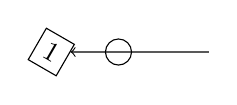
\begin{tikzpicture}[save nodes to file]
\node[draw,rotate=-30,save node](1) at (-2,0) {1};
\draw[->] (0,0) -- (1);
\node[draw,ellipse,save node] (c) at (current bounding box.center) {};
\end{tikzpicture}
\end{document}
\end{filecontents}

%% file2.tex
\begin{filecontents}{\jobname-2.tex}
\RequirePackage{luatex85}
\documentclass[tikz,border=10pt]{standalone}
\usetikzlibrary{tikzmark,shapes.geometric}
\begin{document}
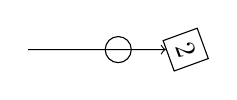
\begin{tikzpicture}[save nodes to file]
\node[draw,rotate=-70,save node] (2) at (2,0) {2};
\draw[->] (0,0) -- (2);
\node[draw,ellipse,save node] (c) at (current bounding box.center) {};
\end{tikzpicture}
\end{document}
\end{filecontents}

%% file3.tex

\immediate\write18{lualatex \jobname-1.tex}
\immediate\write18{lualatex \jobname-2.tex}

\begin{document}
\begin{tikzpicture}

\node[draw,
  rotate=30,
  restore nodes from file={[transform saved nodes,name prefix=pic-1-]{\jobname-1}}
] (a-1) at (-2,-3) {\includegraphics{\jobname-1.pdf}};

\node[draw,
  rotate=70,
  restore nodes from file={[transform saved nodes,name prefix=pic-2-]{\jobname-2}}
] (a-2) at (+2,+2) {\includegraphics{\jobname-2.pdf}};

\draw[red] (pic-1-1.north west) --  (pic-1-1.north east) --  (pic-1-1.south east) --  (pic-1-1.south west) -- cycle;
\draw[red] (pic-2-2.north west) --  (pic-2-2.north east) --  (pic-2-2.south east) --  (pic-2-2.south west) -- cycle;

\node[red] at (pic-1-1) {1};
\node[red] at (pic-2-2) {2};

\draw (a-1) circle[radius=5pt];
\draw (a-2) circle[radius=5pt];

\draw (pic-1-1) -- (pic-2-2);
\end{tikzpicture}
\end{document}
